\chapter{}
Em junho de 1979, papai faleceu.
Um ano antes, aos trinta e dois anos de vida, ainda recebi dele uma última lição.
 
Era julho, eu estava grávida do Vicente que nasceria em outubro e o sobrado que alugávamos próximo da fábrica revelara-se insalubre para as crianças, por conta de um vazamento sob o alicerce que impregnava suas paredes de umidade e também por causa de uma fumaça ácida lançada pelas chaminés da fábrica de suco de laranja, ali perto, que assentava na baixada onde se situava nossa casa, provocando toda sorte de alergias respiratórias.

Isoladamente, as coisas que me afetavam naquele momento, seriam suportáveis.
Após deixar Alta Floresta, para ficar perto de casa, Paulo tinha arrendado uma área de terra em Araraquara.
Insistia ainda na ideia de produzir sementes certificadas de amendoim.
O cultivo vicejou, maravilhoso, mas, de novo, a chuva atrapalhou.
A colheita se perdeu.
Ficamos cheios de dívidas e tivemos que desistir também desta fazenda.
Felizmente, um convite veio de Jaú, a cerca de sessenta quilômetros de Araraquara, para que Paulo gerenciasse uma cooperativa de plantadores de café.
Embora ele tivesse que passar fora o dia todo, poderia vir dormir em casa todas as noites.
Foi um alívio.
Mas, eu ainda lecionava, Tomaz tinha apenas seis anos e o outros três vinham logo abaixo, em escadinha, e uma temporada de doenças sucessivas dos meninos somadas às crises de saúde do papai que se amiudavam, estavam me levando ao esgotamento.
 
Quando meus pais se mudaram para um apartamento, a antiga casa deles passou a ser usada pela minha irmã, enquanto a dela passava por reformas.
Papai sugerira que, assim que ela saísse, eu fosse para lá com minha família, pois a casa ficava num bairro mais alto, mais ensolarado e mais saudável.
Ocorre que a reforma do Renatão parecia interminável e eu estava vendo que meu filho ia nascer naquele maldito sobrado e seria mais um a frequentar semanalmente o consultório médico.

Um dia em que conversava com papai no sítio, meio exasperada, cobrei dele que apressasse meu cunhado.
Ele então quis saber o que me conferia o direito de fazer tal exigência.
Olhei-o entre magoada e chocada.
Afinal, será que ele não via o meu barrigão, o meu rosto abatido, as minhas olheiras de noites e noites mal dormidas, algumas até exatamente por causa dele? Foi daí que ouvi:
\textit{``-- A casa é minha.
Eu tenho direito sobre ela porque a construí com o meu trabalho.
Você, não.
Para o seu bem, vou lhe ensinar ainda uma vez: direito se conquista, não se exige.
Se quer ter direitos, vá embora com seu marido, trabalhe ao lado dele, construa seu próprio patrimônio.
Aí vai poder, sobre o que lhe pertence legitimamente, exigir o que quiser.''}

Não gosto de me ver diminuída assim e quando isso acontece, apesar da raiva, minha reação imediata é descobrir como e por que me expus a ser rebaixada.
Meu pai, mesmo alterado pela bebida, e era o caso naquele dia, não costumava errar na avaliação dos motivos do outro.
A custo, tive que admitir que, no fundo, ele tinha razão.
Envergonhada, perguntei a mim mesma se me acreditava credora de recompensa por estar ajudando meus pais naquela provação em que a doença dele se transformara.
Ou, o mais provável, se por baixo do louvável e sincero sentimento de compromisso filial, não se insinuava também aquele medo habitual e covarde de assumir minha própria vida que com certeza colaborava para que eu protelasse a decisão de seguir meu marido.
Eu sabia a resposta e por isso decidi que, quando meu pai morresse, eu me obrigaria a ir com Paulo para onde quer que fosse.
Até porque eu lhe devia esse gesto, pela paciência e a compreensão que demonstrara ao longo de tantos anos em que me recusei a acompanhá-lo.

Apesar do que havia me dito, meu pai, como era do feitio dele, assim que a família da Maria Lúcia se mudou, rapidamente arrumou e reformou toda a sua antiga casa, de modo que quando voltei da maternidade com Vicente, pudemos nos instalar lá.


\begin{figure}
\centering
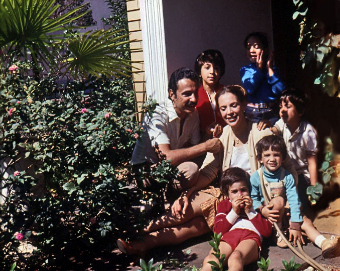
\includegraphics[width=0.8\linewidth]{29/na-casa.png}
\caption{Na casa da avenida D.Pedro II, pouco antes da mudança para Conceição.}
\end{figure}

Pouco menos de um ano depois, o Comandante teve, pela segunda vez, um grave edema de pulmão.
Os irmãos médicos vieram do Rio para visitá-lo.
Na véspera do dia em que retornariam, Tio Ângelo, o mais velho, chamou-me lá fora, no corredor do hospital:

\textit{``-- Teresa, seu pai está no fim.
Os exames mostram cerca de noventa por cento do coração necrosado pelos muitos enfartes.
Tem, quando muito, uma semana ou dez dias de vida.
Prepare-se e prepare sua mãe.''}

\textit{``-- Há risco de que seja por edema, com todo aquele sofrimento pela terceira vez?''}, eu quis saber.

\textit{``-- Não creio.
O coração está tão fraco que não suportará qualquer esforço maior.
Entrará em choque antes, se isso consola você.''}

Voltei ao quarto, incrédula.
Meu pai parecia tão bem, depois do susto.
No hospital, sem poder beber nem fumar, ele voltava a ser o Mathias dos bons tempos.

\begin{figure}
\centering
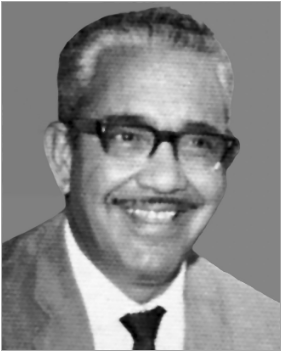
\includegraphics[width=\linewidth]{29/papai.png}
\caption{Papai, por volta dos sessenta anos.}
\end{figure}

Uma semana depois, logo de manhã, vendo-se banhado, penteado e barbeado, ele comentou sorrindo:

\textit{``-- Agora estou pronto para o caixão.
Limpinho e arrumadinho.''}

\textit{``-- Não diga bobagem, Mathias''}, retrucou minha mãe que ia saindo para dar um pulo até o apartamento deles, ali perto, a menos de meio quarteirão.

Mamãe não chegou a tomar o elevador.
Vieram chamá-la correndo porque meu pai acabara de ter um enfarte.
O derradeiro.
Cheguei quase em seguida.
Haviam-no deitado sobre um lençol, no chão, para tentar reanimá-lo.
Parecia grande e sólido como um jequitibá tombado.
Após longos minutos de luta infrutífera, mamãe e eu pedimos aos médicos: 

\textit{``-- Deixem-no ir.
Ele precisa descansar.''}

Ele já não estava mais ali.
Desde aquele momento acreditei que para onde quer que tenha ido, haveria de estar no lugar destinado aos justos.
Porque estourara até a última fibra daquele coração na luta para ir além de si mesmo, das suas fraquezas, das suas inseguranças e dos seus desejos, por nós e por todos que dele precisaram nessa vida.

Todavia, voltando a me lembrar do que me ensinou o velho jesuíta, o problema das grandes árvores é que à sombra delas, as outras plantas minguam.
Desaparecido o Comandante, todos nós teríamos que crescer e esse crescimento seria terrivelmente doloroso.

Papai morreu em 6 de junho de 1979.
Vicente tinha nascido alguns meses antes, em 2 de outubro de 1978.

Eu sempre lutava para continuar dando aulas até onde aguentasse, para poder usufruir a licença gestante completa após a chegada do bebê.
Daí que um dia, ao fim do nono mês de gestação, após dar minha última aula da manhã, resolvi passar rapidamente por uma liquidação numa loja de departamentos no centro da cidade.
Vicente estava para chegar e, sendo o quinto, já pouco ou nada restava dos enxovais anteriores.
Assim que comecei a separar as peças que me interessavam, percebi, pelo alarme estampado no rosto da vendedora, que minha aparência devia estar bem estranha.
Já fazia um calor enorme naquele outubro e a loja estava lotada.
Ela correu para buscar uma cadeira.
Não deu tempo.
Quando chegou de volta, eu estava plantada no centro de um lago de líquido amniótico.
A bolsa rompera.
Por sorte, Dr. Elias me esperava no hospital, ali ao lado, para fazer o último ultrassom que estabeleceria o dia aproximado do parto.
Não foi preciso.
Vicente nasceu uma hora depois.
De brincadeira, as meninas do berçário fizeram questão de trazê-lo ao quarto todo pimpão, de roupinhas novas, ostentando por todo lado as coloridas etiquetas da remarcação.


\begin{figure}
\centering
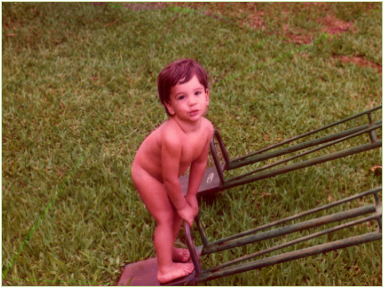
\includegraphics[width=0.8\linewidth]{29/vicente.png}
\caption{Vicente, no seu primeiro ano de vida}
\end{figure}

\begin{figure}
\centering
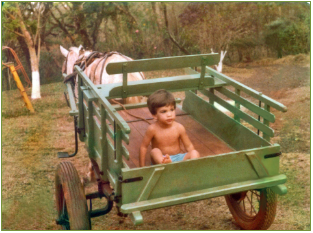
\includegraphics[width=0.8\linewidth]{29/vicente-pensativo.png}
\caption{Pensativo, como sempre}
\end{figure}

Ainda ficamos por quase dois anos em Araraquara.
No momento em que o rochedo à sombra do qual se sentia segura deixou de existir, Lectícia entrou em pânico e, com um único gesto, quase implodiu a família: ungiu Reginaldo, seu filho mais velho como sucessor do pai e delegou-lhe autoridade para tomar decisões em nome dela.
Até aí, o gesto pareceria natural, não fosse o fato de que havia mais dois filhos homens numa idade especialmente sensível e que, por esse decreto, ficavam automaticamente submetidos à autoridade do irmão mais velho e, pior, convencidos em definitivo de que o que até então havia sido para eles mera suspeita, confirmara-se como clara verdade: Reginaldo era o filho predileto dela, o único em quem ela confiava.
Isso sem falar no resto da família, filhas e cunhados, nem cheirados e nem ouvidos e que foram igualmente postos em desconfiança.
Papai, antes de morrer, já prevendo a catástrofe, havia feito uma tentativa frustrada de unir filhos homens e cunhados numa espécie de comitê gestor dos negócios.
Mas logo percebeu que Paulo, com a inquietude que lhe era característica, não levaria muito longe um compromisso dessa espécie.
Já Reginaldo, de natureza autocrática, pouco afeito a delegar ou partilhar o que quer que fosse, dificilmente se combinaria com o matreiro Renato e, verdade seja dita, na hora mesmo ele tratou de deixar isso claro: se tivesse que assumir, seria sozinho.

Lembro-me de ter escrito uma carta ao meu irmão, advertindo-o sobre o risco de aceitar uma imposição irracional saída da cabeça de uma Lectícia fragilizada pelo único medo que ela conhecia: o medo de voltar a ser pobre.
Mas o fato de eu ser uma das herdeiras preteridas e considerada naquele momento a menos bem sucedida financeiramente, não conferia autoridade ao que eu dissesse naquela hora.
Tentar alertar mamãe para o futuro que se desenhava a partir da sua atitude intempestiva, nem pensar.
Ela se descontrolava à simples menção do assunto.
De qualquer modo, meu irmão Paulinho ainda era menor de idade e nenhum passo relativo ao inventário poderia ser dado antes que ele atingisse a maioridade.
Só restava torcer para que o estrago não fosse muito grande até que esse momento chegasse e para que minha mãe, com o passar do tempo, recuperasse o domínio sobre si mesma.

Em 1981, Paulo passou seis meses em Belém do Pará fazendo uma especialização em Heveicultura.
Os irmãos Gomes dos Reis, associados da cooperativa, convidaram-no a gerenciar a implantação de um cultivo de seringueira financiado pela SUDAM\footnote{Superintendência do Desenvolvimento da Amazônia, uma autarquia.} nas propriedades que possuíam no Pará, no município de Conceição do Araguaia e, para tanto, acharam conveniente proporcionar-lhe uma formação mais específica no assunto.
A promessa era de que, para complementar salário, o grupo doaria ao meu marido uma pequena parte das suas extensas terras, onde ele poderia instalar o seu próprio seringal